\section{Introduction}
\label{sec:introduction_f}



With the advent of smart conversational agents such as Amazon Alexa, Google Assistant, etc., dialogue systems are becoming ubiquitous. 
In the context of enterprises, the majority of these systems target task oriented dialogues with the user trying to achieve a goal, e.g. booking flight tickets or ordering food. \textcolor{black}{Natural Language Understanding (NLU) captures the semantic meaning of a user's utterance within each dialogue turn, by identifying \textbf{intents} and \textbf{slots}. }
An intent specifies the goal underlying the expressed utterance while slots are additional parameters for these intents. These tasks are typically articulated as intent classification (\pretty{IC}) coupled with
sequence tagging task of slot labeling (\pretty{SL}).
%sequence labeling \peng{and} \peng{\st{similar to named entity recognition (NER), for}} slot labeling (SL). 

\begin{figure}[t]
\centering
% <PLACEHOLDER for NEW DIAGRAM>
%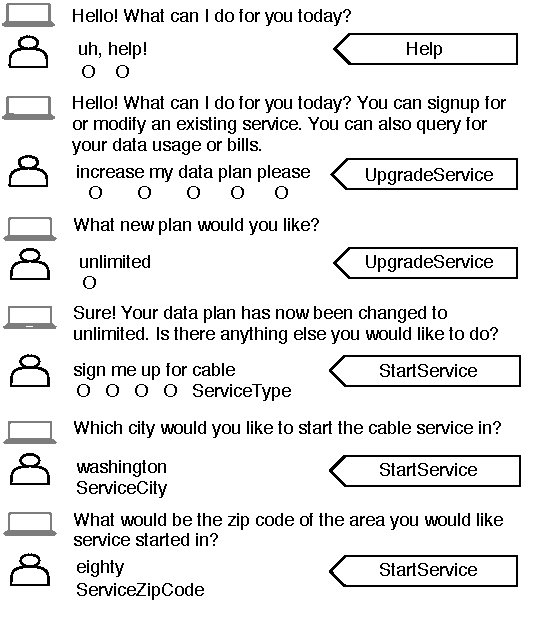
\includegraphics[width=200pt, height=150pt, width=0.5\textwidth]{figures/dialog_example.pdf}
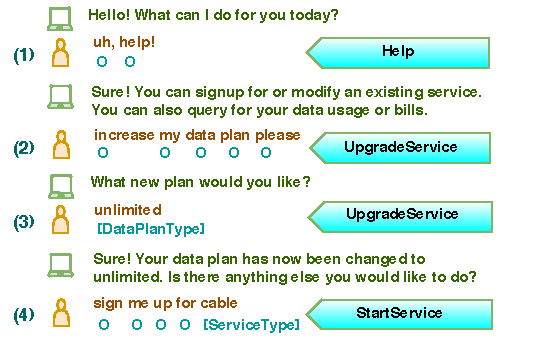
\includegraphics[width=150pt, height=120pt, width=0.5\textwidth]{figures/dialog_example_v17.pdf}
\vspace{-20pt}
\caption{\label{tease} \small Snippet of a sample Cable data conversation with intents shown in boxes and slots aligned with user request}%%Garima, I would modify the second prompt *not* to have the "Hello! What can i do for you today?" portion. Start the prompt from "You can signup ..." or better yet something like "Sure! You can signup..."
%%Done
\vspace{-20pt}
\end{figure}


Over time, human-machine interactions have become more complex with greater reliance on contextual cues for utterance understanding 
% especially in multi-goal (multiple intents fulfillment) conversations 
(Figure \ref{tease}).
%With progress in the field of modeling human-machine interactions, conversations are getting more complex and thus relying more on contextual cues to interpret the utterances.
With traditional NLU frameworks, the resolution of contextual utterances is typically addressed in the DM component of the system using rule-based dialogue state trackers (\pretty{DST}). However, this pushes the problem of context resolution further down the dialogue pipeline, and despite the appeal of modularity in design, it opens the door for significant cascade of errors. To avoid this, end-to-end dialogue systems have been proposed \cite{wen_end2end, end2end_goal}, but, to date, such systems are not scalable in industrial settings, and tend to be opaque where a level of transparency is needed, for instance, to understand various dialogue policies. 

To address %\glalwani{\sout{some of}}
the propagation of error while maintaining a modular 
%\st{and interpretable} 
framework, \citet{Shi2015ContextualSL} %TODO: We can add more references here
proposed adding contextual signals to the joint IC-SL task. However, \textcolor{black}{the contributions of }their work were limited in terms of number of signals and how they were used, rendering the contextualization process still less interpretable. In this work, we present a multi-dimensional self-attention based contextual NLU model that overcomes prior work's shortcomings by supporting variable number of contextual signals (previous utterances, dialogue acts\footnote{Dialog Act signifies the actions taken by the agent such as Close (when an intent is fulfilled), ElicitSlot, etc}, intents and slot labels) that can be used concurrently over variable length of conversation context.
%\sout{In this work, we present a multi-dimensional self-attention based contextual \pretty{Nlu} model that supports variable number of contextual signals (previous utterances, dialogue acts\footnote{Dialog Act signifies the actions taken by the agent such as Close (when an intent is fulfilled), ElicitSlot, etc}, intents and slot labels) over a variable length of context, that can be concurrently used for the task while overcoming the prior works' short-comings.}
In addition, our model allows for easy visualization and debugging of contextual signals which are essential, especially in production dialogue systems, where interpretability is a desirable feature. Our contributions are:
\begin{itemize}[noitemsep,topsep=0pt,parsep=0pt,partopsep=0pt]
\item Context-Aware Self-Attentive NLU (\pretty{Casa-NLU}) model that uses various contextual signals to perform joint IC-SL task, outperforming contextual and non-contextual NLU baselines by significant margins on two in-house conversational IC-SL datasets
\item Propose a novel non-contextual variant of \pretty{Casa-nlu} that achieves SOTA performance on IC task for both \pretty{Snips} and \pretty{ATIS} datasets
\item Analysis of the various contextual signals' contributions to model performance
\end{itemize}



